\section{Evaluation of NRSfM}
\frame{
  \frametitle{A Benchmark and Evaluation of Non-Rigid Structure from Motion}
  Sebastian Hoppe Nesgaard Jensen, Alessio Del Bue, Mads Emil Brix Doest and Henrik Aanæs

  \textit{IEEE Transactions on Pattern Analysis and Machine Intelligence (Under review)}
  \begin{figure}
    \centering
    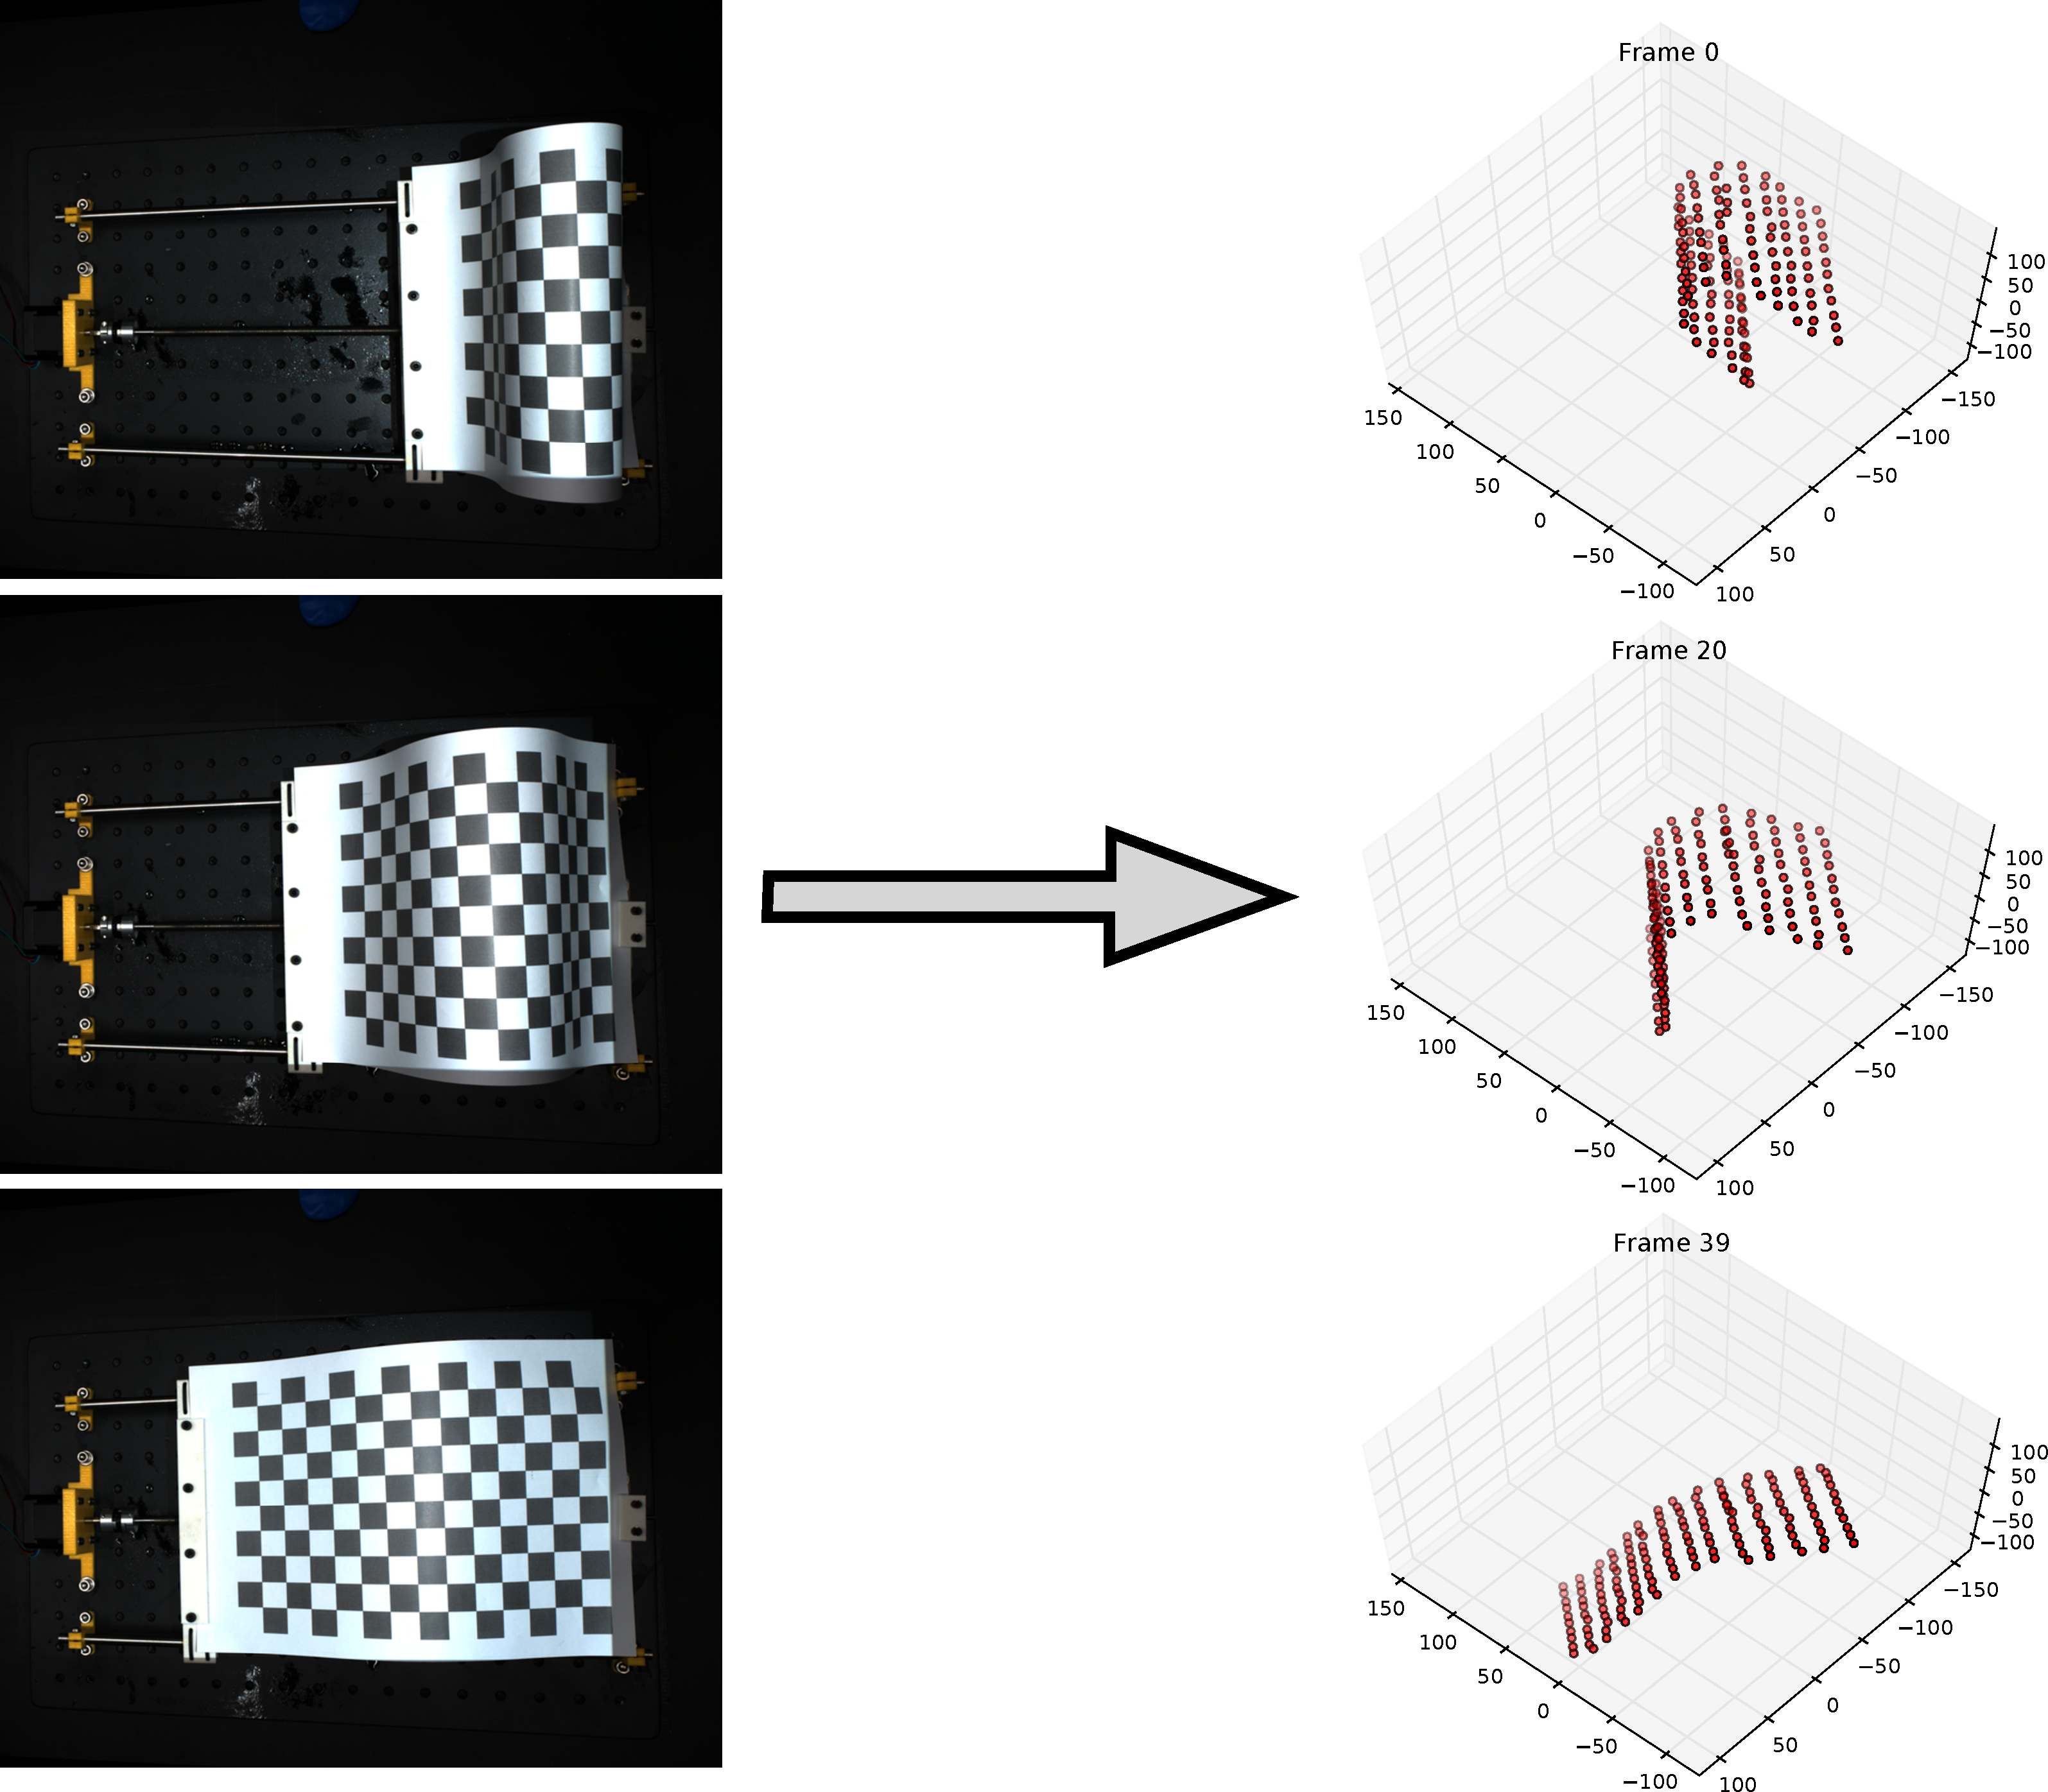
\includegraphics[height=0.65\textheight]{figures/nrsfm_paper_idea}
  \end{figure}
}

\frame{
  \frametitle{Structure-from-Motion}
  %\begin{figure}
  \begin{minipage}{0.48\textwidth}
    \begin{figure}
      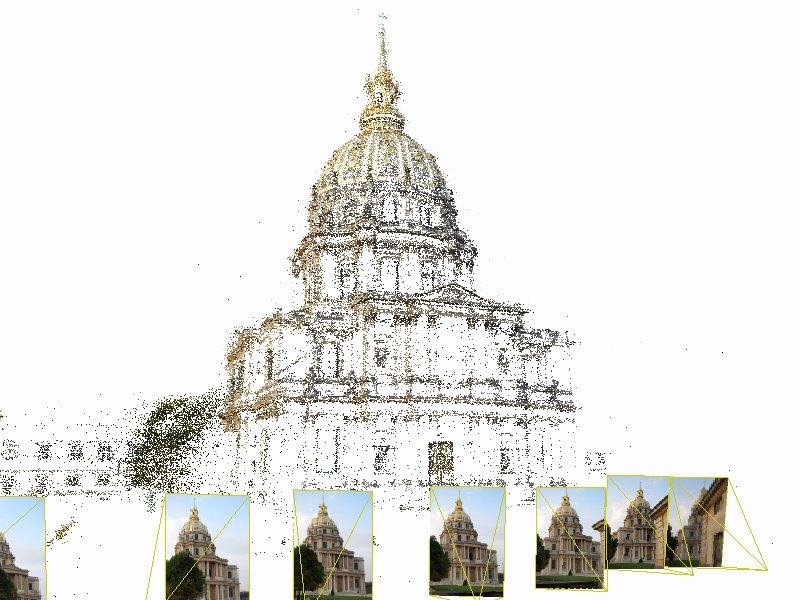
\includegraphics[height=0.65\textheight]{figures/sfm_0}
      \caption{\cite{enqvist2010stable}}
    \end{figure}
  \end{minipage}
  \hfill
  \begin{minipage}{0.48\textwidth}
    \begin{figure}
      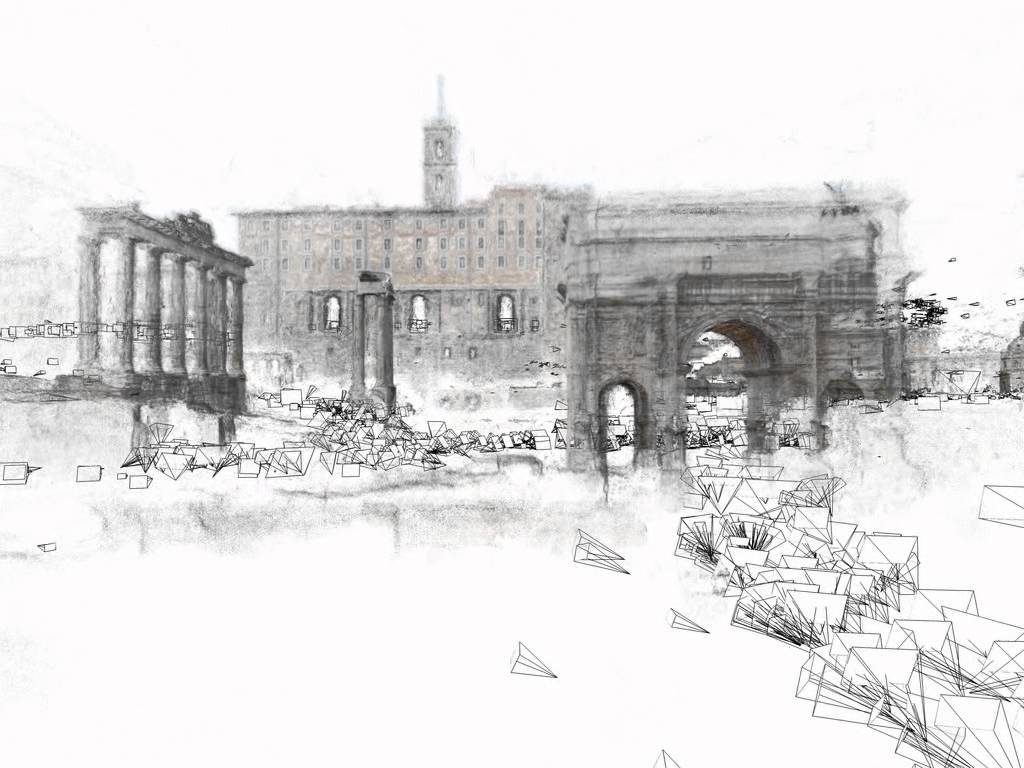
\includegraphics[height=0.65\textheight]{figures/sfm_1}
      \caption{\cite{crandall2011discrete}}
    \end{figure}
  \end{minipage}
  %\end{figure}
}

\frame{
  \frametitle{Factorization of Structure-from-Motion}
  Assuming orthographic projection,
  \begin{align}
    \mathbf{W} = \mathbf{M}\mathbf{S}    \label{eq:nrsfm_fac}
  \end{align}
  \begin{align*}
    \mathbf{W} = \begin{bmatrix}
      \mathbf{w}_{11} & \mathbf{w}_{12} & \cdots & \mathbf{w}_{1P}\\
      \mathbf{w}_{21} & \mathbf{w}_{22} & \cdots & \mathbf{w}_{2P}\\
      \vdots   & \vdots   & \ddots & \vdots\\
      \mathbf{w}_{F1} & \mathbf{w}_{F2} & \cdots & \mathbf{w}_{FP}
    \end{bmatrix},
    \mathbf{M} = \begin{bmatrix}
      \mathbf{M}_1 & \mathbf{0}   & \cdots & \mathbf{0}\\
      \mathbf{0}   & \mathbf{M}_2 & \cdots & \mathbf{0}\\
      \vdots       & \vdots       & \ddots & \vdots    \\
      \mathbf{0}   & \mathbf{0}   & \cdots & \mathbf{M}_F
    \end{bmatrix},
    \mathbf{S} = \begin{bmatrix}
      \mathbf{s}_{11} & \mathbf{s}_{12} & \cdots & \mathbf{s}_{1P}\\
      \mathbf{s}_{21} & \mathbf{s}_{22} & \cdots & \mathbf{s}_{2P}\\
      \vdots       & \vdots       & \ddots & \vdots    \\
      \mathbf{s}_{F1} & \mathbf{s}_{F2} & \cdots & \mathbf{s}_{FP}
    \end{bmatrix}
  \end{align*}
}

\frame{
  \frametitle{Not Much Concensus on the Best Approach}
  \begin{minipage}{0.48\textwidth}
    \begin{itemize}
      \item Low-rank basis
      \item DCT coefficients
      \item Spatial and temporal
      \item Clustering
      \item Perspective correction
      \item Compressibility
      \item And much more...
    \end{itemize}
  \end{minipage}
  \begin{minipage}{0.48\textwidth}
    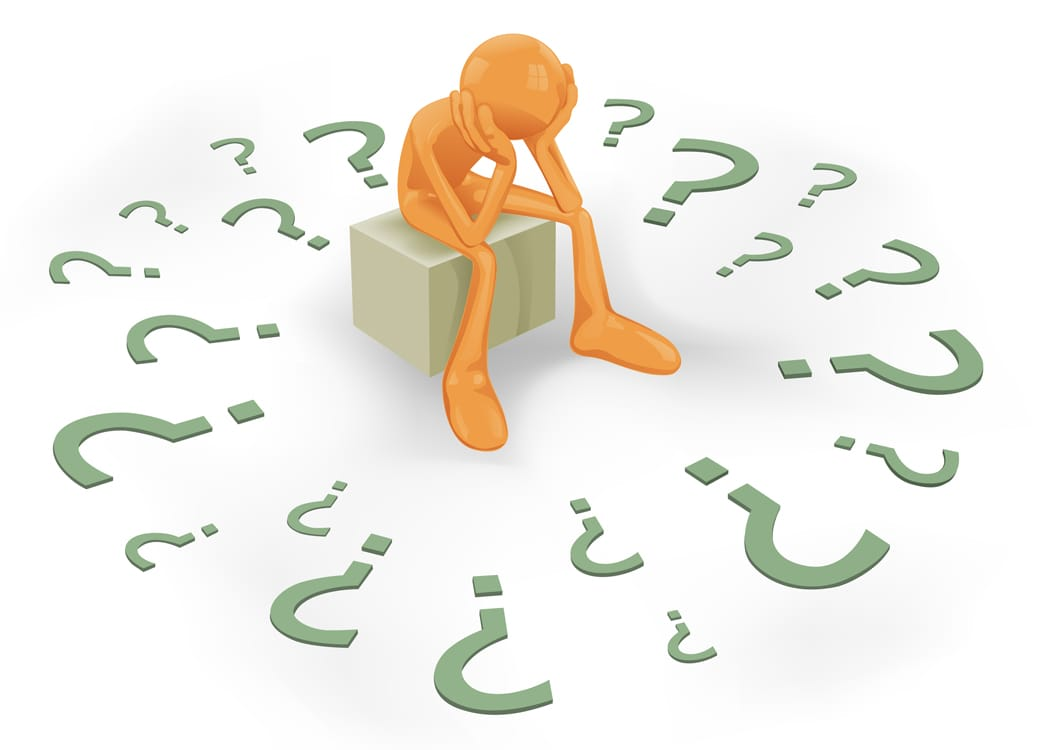
\includegraphics[width=\textwidth]{figures/confusion}
  \end{minipage}
}

\frame{
  \frametitle{Previous Datasets}
  \begin{center}
    \movie[autostart, loop, width = 0.48\textwidth, height = 0.8\textheight, poster]{}{videos/shark.avi}
    \hfill
    \movie[autostart, loop, width = 0.48\textwidth, height = 0.8\textheight, poster]{}{videos/walk.avi}
  \end{center}
  Animations and motion capture.
}

\frame{
  \frametitle{Important Questions}
  \begin{itemize}
    \item Which algorithms gives the best results on average?
    %\item Which types motions are the most difficult to reconstruct?
    \item How are missing observations best dealt with?
    \item How important is the assumption of an orthographic camera?
  \end{itemize}
}

\frame{
  \frametitle{Inspiration: Stop-Motion}
  \movie[autostart, loop, width = 0.48\textwidth, height = 0.7\textheight, poster]{}{videos/skeleton.avi}
  \hfill
  \movie[autostart, loop, width = 0.48\textwidth, height = 0.7\textheight, poster]{}{videos/wallace.avi}
}

\frame{
  \movie[autostart, loop, width = 0.32\textwidth, height = 0.48\textheight]{}{videos/articulated/output.avi}
  \movie[autostart, loop, width = 0.32\textwidth, height = 0.48\textheight]{}{videos/balloon/output.avi}
  \movie[autostart, loop, width = 0.32\textwidth, height = 0.48\textheight]{}{videos/paper/output.avi}
  %\movie[autostart, loop, width = 0.32\textwidth, height = 0.48\textheight]{}{videos/paper.avi}
  %\movie[autostart, loop, width = 0.32\textwidth, height = 0.48\textheight]{}{videos/balloon.avi}
  \begin{center}
    \movie[autostart, loop, width = 0.32\textwidth, height = 0.48\textheight]{}{videos/stretch/output.avi}
    \movie[autostart, loop, width = 0.32\textwidth, height = 0.48\textheight]{}{videos/tear/output.avi}
  \end{center}
}

\frame{
  \frametitle{Recording Setup}
  \includegraphics[height = 0.7\textheight]{figures/nrsfm_cell}
  \hfill
  \includegraphics[height = 0.7\textheight]{figures/nrsfm_scanner}
}

\frame{
  \frametitle{Virtual Camera Paths}
  \begin{center}
    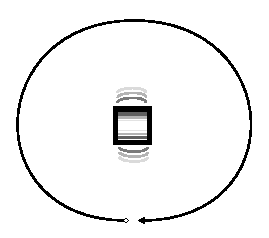
\includegraphics[height = 0.45\textheight]{figures/circle}
    \hfill
    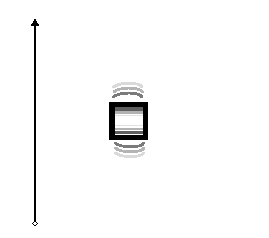
\includegraphics[height = 0.45\textheight]{figures/line}
    \hfill
    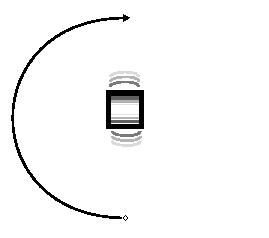
\includegraphics[height = 0.45\textheight]{figures/half_circle}
  \end{center}
  \begin{center}
    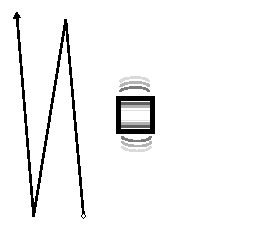
\includegraphics[height = 0.45\textheight]{figures/zigzag}
    \hfill
    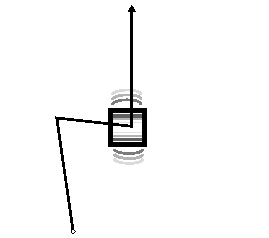
\includegraphics[height = 0.45\textheight]{figures/flyby}
    \hfill
    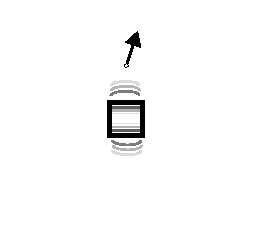
\includegraphics[height = 0.45\textheight]{figures/tricky}
  \end{center}
}

\frame{
  \frametitle{Observations}
  \begin{center}
    \movie[autostart, loop, width = 0.32\textwidth, height = 0.48\textheight]{}{videos/observations/circle/output.avi}
    \hfill
    \movie[autostart, loop, width = 0.32\textwidth, height = 0.48\textheight]{}{videos/observations/line/output.avi}
    \hfill
    \movie[autostart, loop, width = 0.32\textwidth, height = 0.48\textheight]{}{videos/observations/semi/output.avi}
  \end{center}
  \begin{center}
    \movie[autostart, loop, width = 0.32\textwidth, height = 0.48\textheight]{}{videos/observations/zigzag/output.avi}
    \hfill
    \movie[autostart, loop, width = 0.32\textwidth, height = 0.48\textheight]{}{videos/observations/flyby/output.avi}
    \hfill
    \movie[autostart, loop, width = 0.32\textwidth, height = 0.48\textheight]{}{videos/observations/tricky/output.avi}
  \end{center}
}

\frame{
  \frametitle{Missing Observations}
  \begin{center}
    \movie[autostart, loop, width = 0.32\textwidth, height = 0.48\textheight]{}{videos/missingdata/circle/output.avi}
    \hfill
    \movie[autostart, loop, width = 0.32\textwidth, height = 0.48\textheight]{}{videos/missingdata/line/output.avi}
    \hfill
    \movie[autostart, loop, width = 0.32\textwidth, height = 0.48\textheight]{}{videos/missingdata/semi/output.avi}
  \end{center}
  \begin{center}
    \movie[autostart, loop, width = 0.32\textwidth, height = 0.48\textheight]{}{videos/missingdata/zigzag/output.avi}
    \hfill
    \movie[autostart, loop, width = 0.32\textwidth, height = 0.48\textheight]{}{videos/missingdata/flyby/output.avi}
    \hfill
    \movie[autostart, loop, width = 0.32\textwidth, height = 0.48\textheight]{}{videos/missingdata/tricky/output.avi}
  \end{center}
}

\frame{
  \frametitle{Algorithm Performance without Missing Observations}
  \begin{table}[!t]
  \centering
  %\caption{Averages given in milimeters.}
  %\label{table:full_linear_algo}

  \begin{tabular}{r r r r}\toprule
    \textbf{MultiBody} & \textbf{KSTA} & \textbf{RIKS} & \textbf{CSF2}\\
    29.36 & 31.94 & 32.21 & 32.83\\ \midrule
    \textbf{MetricProj} & \textbf{CSF} & \textbf{Bundle} & \textbf{PTA}\\
    34.09 & 41.19 & 46.66 & 46.80\\ \midrule
    \textbf{ScalableSurface} & \textbf{EM PPCA} & \textbf{SoftInext} & \textbf{BALM}\\
    53.88 & 59.19 & 61.94 & 66.34\\ \midrule
    \textbf{MDH} & \textbf{Compressible} & \textbf{SPFM} & \textbf{Consensus}\\
    70.34 & 79.18 & 85.34 & 94.61\\ \midrule
  \end{tabular}
\end{table}
Numbers are averages given in milimeters.
}

\frame{
  \frametitle{Error Distribution of the Top Five Algorithms}
  \begin{center}
    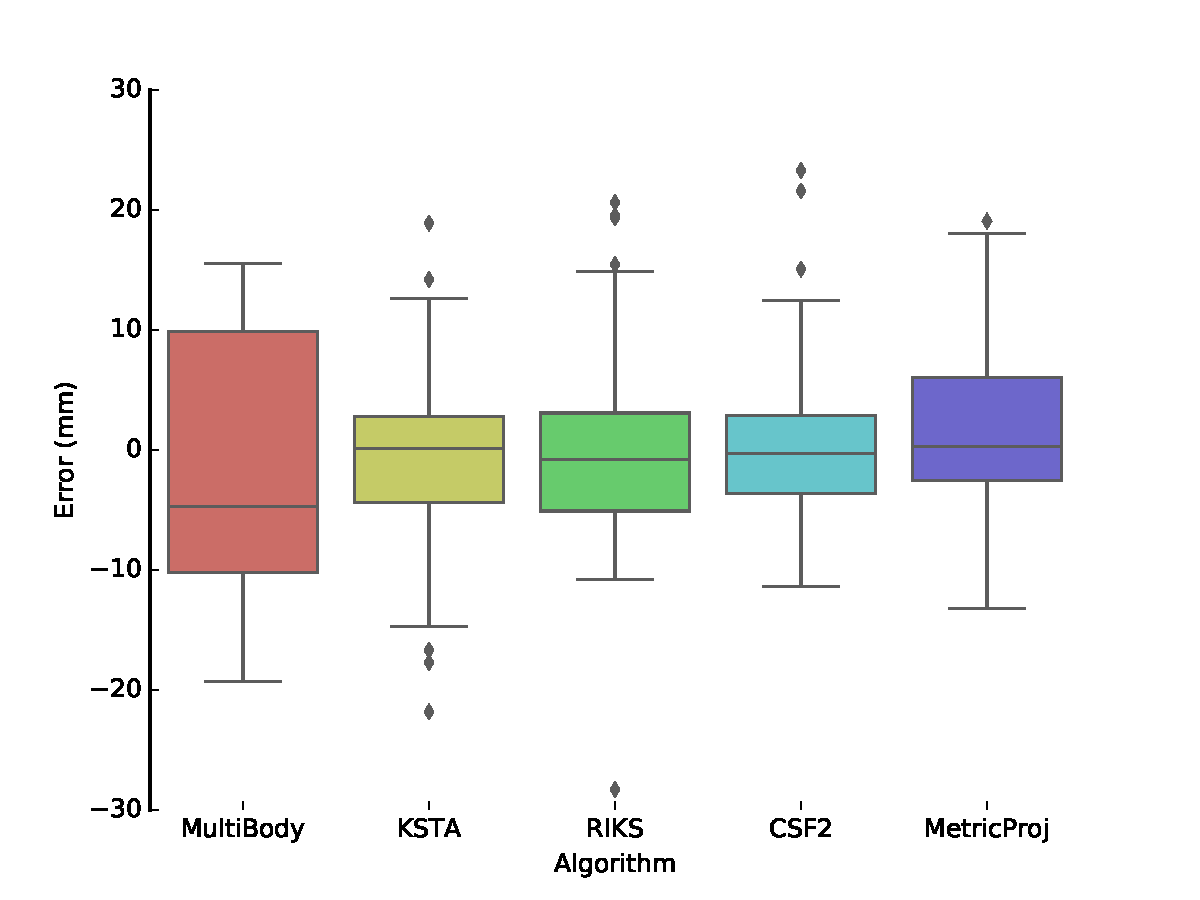
\includegraphics[height = 0.8\textheight]{figures/algo_box}
  \end{center}
  Adjusted for influence of other factors such as camera model, deformation type etc.
}

\frame{
  \frametitle{Influence of Missing Observations}
  \begin{center}
    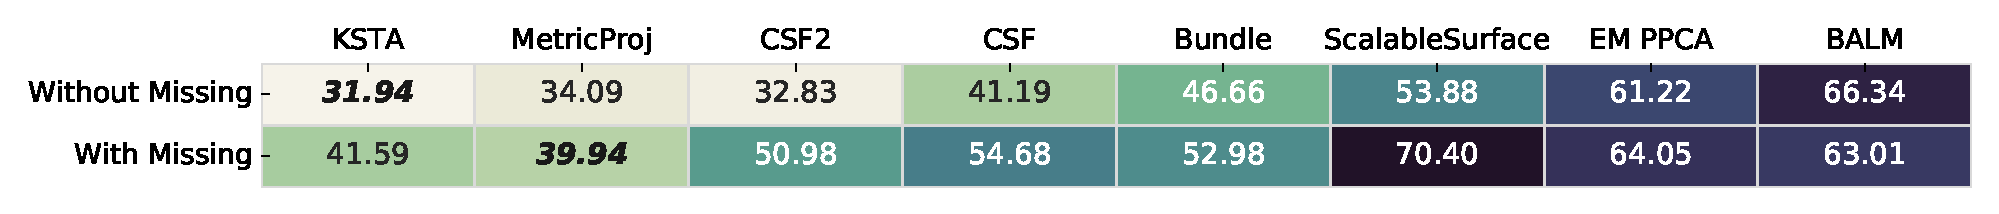
\includegraphics[width = \textwidth]{figures/miss_algo}
  \end{center}
  Numbers are averages given in milimeters.
}

\frame{
  \frametitle{Influence of the Camera Model}
  \begin{center}
    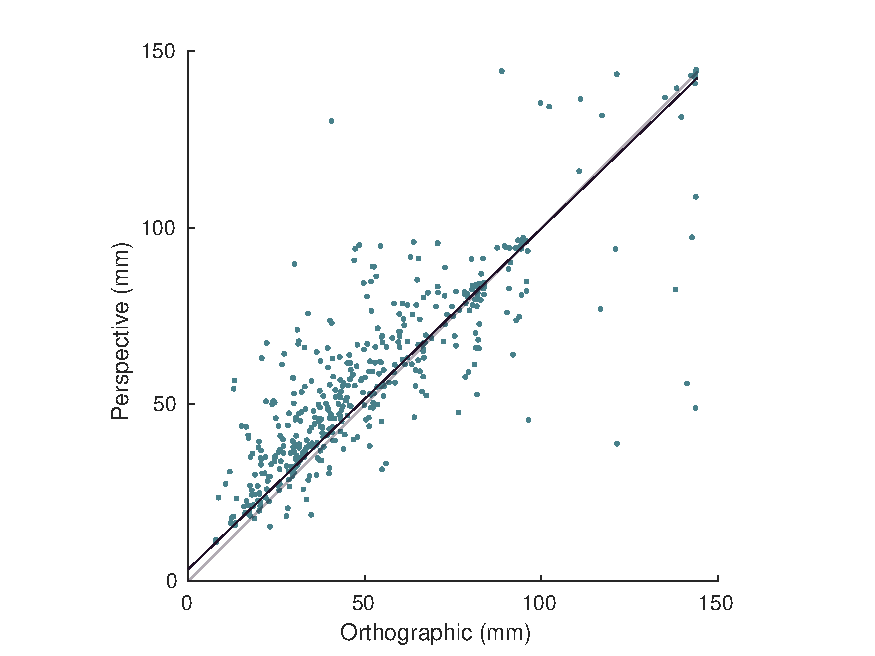
\includegraphics[height = 0.8\textheight]{figures/ort_per_scatter}
  \end{center}
  Repeated experiments with different camera models. Fitted a line gives $y = 0.96x + 4.06$. ANOVA indicates a mean increase in error of $7.2mm$. 
}

\frame{
  \frametitle{Conclusion}
  \begin{itemize}
    \item Created a varied dataset with groundtruth and realistic missing observations.
    \item Established ranking of NRSfM algorithms.
    \item Many methods are unable to handle occlusion-based missing observations.
    \item Orthographic camera assumption does not break under perspective projection.
  \end{itemize}
  Consider implementing Metric Proj. matrix completion algorithm for filling missing observations.
}
